% Created 2020-08-14 ven 17:00
% Intended LaTeX compiler: pdflatex
\documentclass[11pt]{article}
\usepackage[utf8]{inputenc}
\usepackage[T1]{fontenc}
\usepackage{graphicx}
\usepackage{grffile}
\usepackage{longtable}
\usepackage{wrapfig}
\usepackage{rotating}
\usepackage[normalem]{ulem}
\usepackage{amsmath}
\usepackage{textcomp}
\usepackage{amssymb}
\usepackage{capt-of}
\usepackage{hyperref}
\author{Eros Zaupa}
\date{\today}
\title{Automating AI lifecycle: the DDoS use case}
\hypersetup{
 pdfauthor={Eros Zaupa},
 pdftitle={Automating AI lifecycle: the DDoS use case},
 pdfkeywords={},
 pdfsubject={},
 pdfcreator={Emacs 26.3 (Org mode 9.1.9)}, 
 pdflang={English}}
\begin{document}

\maketitle
\section*{Automating AI lifecycle: the DDoS use case}
\label{sec:orgd378da0}
Eros Zaupa
\section*{Project goals}
\label{sec:orgec83642}
\begin{description}
\item[{CICDDoS2019}] Discover this new dataset for DDoS attacks
\item[{DNN}] Design and develop a classifier using the dataset
\item[{Kubeflow}] Design and develop a ML pipeline for the DNN
\end{description}
\section*{CICDDoS2019}
\label{sec:orge860c77}
\subsection*{Proposed taxonomy}
\label{sec:org544229d}
\begin{center}
\includegraphics[width=.9\linewidth]{https://www.unb.ca/cic/_assets/images/ddostaxonomy.png}
\end{center}  \url{https://www.unb.ca/cic/datasets/ddos-2019.html}
\subsection*{Dataset}
\label{sec:org3a31181}
\begin{description}
\item[{Raw data}] With network traffic and event logs
\item[{CSV files}] More than 80 traffic features extracted from the raw
data
\end{description}
\subsection*{Training dataset}
\label{sec:orga5a844a}
\begin{center}
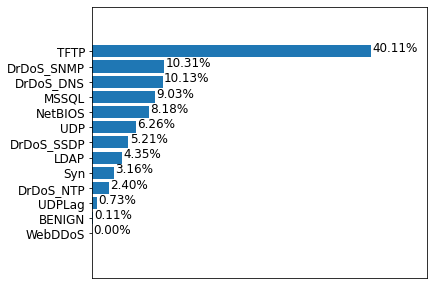
\includegraphics[width=.9\linewidth]{./img/train_ds.png}
\end{center}

Total number of records: 50,063,112
\subsection*{Testing dataset}
\label{sec:org6e00cf0}
\begin{center}
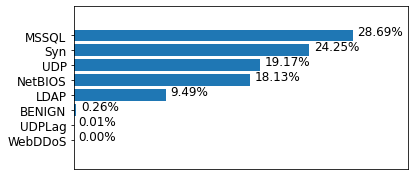
\includegraphics[width=.9\linewidth]{./img/test_ds.png}
\end{center}

Total number of records: 20,172,83
\subsection*{Datasets for DNN}
\label{sec:org61d4a34}
\begin{center}
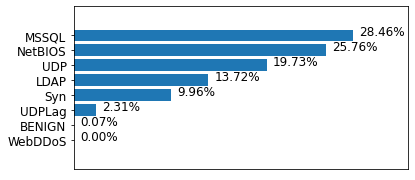
\includegraphics[width=.9\linewidth]{./img/train2_ds.png}
\end{center}
Training dataset

\begin{center}
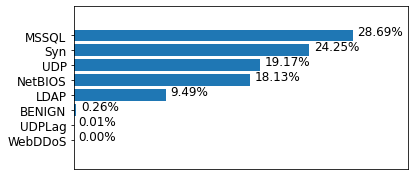
\includegraphics[width=.9\linewidth]{./img/test_ds.png}
\end{center}
Testing dataset

\section*{DNN}
\label{sec:org874ed4c}
\subsection*{Development}
\label{sec:orgf16a172}
\begin{itemize}
\item Python 3.7.7
\begin{itemize}
\item pandas 1.0.3
\item scikit-learn 0.23.1
\end{itemize}
\item Tensorflow 2.1.0
\end{itemize}
\subsection*{Estimators}
\label{sec:orgbe634ca}
\begin{center}
\includegraphics[width=.9\linewidth]{https://miro.medium.com/max/700/1*8e8Aq_GlJFy8tGuZx1F2IA.png}
\end{center}

Tensorflow API stack
\subsection*{Estimator API}
\label{sec:org5b9a733}
\begin{center}
\includegraphics[width=.9\linewidth]{https://miro.medium.com/max/700/1*LF9lKi-LaNRwyL5lLfKRNg.png}
\end{center}

Schematic of Estimator
\subsection*{Design}
\label{sec:org984df0c}
\begin{itemize}
\item Network
\begin{itemize}
\item Dense, feed-forward neural network
\end{itemize}
\item Multiclassification
\begin{itemize}
\item 8 classes
\end{itemize}
\item Features
\begin{itemize}
\item 20 most useful features
\end{itemize}
\item Batch normalization
\item Adam optimizer
\end{itemize}
\subsection*{Hyperparameter tuning}
\label{sec:org15d9683}
\begin{itemize}
\item Number of hidden units
\begin{itemize}
\item\relax [60, 30, 20]
\item\relax [60, 40, 30, 20]
\end{itemize}
\item Dropout rate
\begin{itemize}
\item 0.1
\item 0.2
\end{itemize}
\item Learning rate
\begin{itemize}
\item 0.1
\item 0.3
\end{itemize}
\end{itemize}
\section*{Kubeflow}
\label{sec:orgb42a5cb}
\subsection*{Develoment}
\label{sec:orgf17189a}
\begin{itemize}
\item Docker 18.09.7
\item Kubernetes v1.15.3
\item Kubeflow v1.0
\begin{itemize}
\item Kubeflow Pipeline SDK v1.0.0
\end{itemize}
\end{itemize}
\subsection*{Resources}
\label{sec:org144acd4}
\begin{description}
\item[{Master node}] 4 VCPUs, 8GB RAM, 100GB of storage
\item[{2 x Slave nodes}] 4 VCPUs, 16GB RAM, 100GB of storage
\item[{OS}] Ubuntu 16.04 LTS
\end{description}
\subsection*{Pipelines}
\label{sec:org8381b5d}
\begin{center}
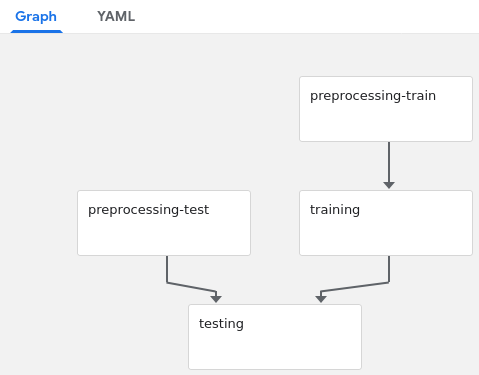
\includegraphics[width=.9\linewidth]{./img/pipeline.png}
\end{center}
\subsection*{Components}
\label{sec:org1a37ef4}
\begin{description}
\item[{Base image}] All the shared dependencies
\begin{description}
\item[{Preprocess-train}] Training dataset + Source code
\item[{Preprocess-test}] Testing dataset + Source code
\item[{Train}] Source code
\item[{Test}] Source code
\end{description}
\end{description}
\subsection*{Experiments}
\label{sec:orge71dd86}
\begin{center}
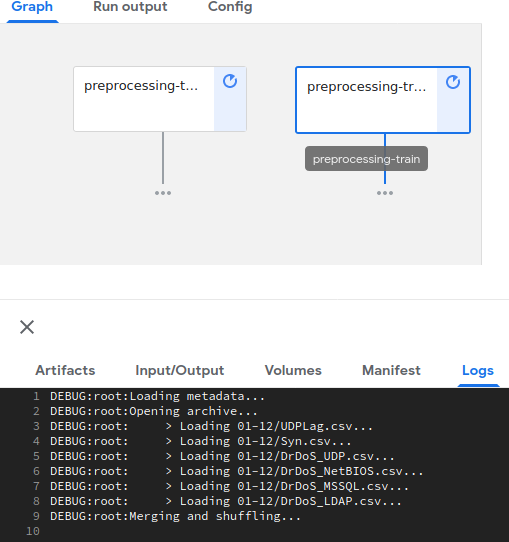
\includegraphics[width=.9\linewidth]{./img/experiment.png}
\end{center}
\subsection*{Behaviour}
\label{sec:org0dba2ce}
\begin{description}
\item[{Load is distribution}] Components are executed according to the
available resources
\item[{Failure}] If any node fails, the experiment is resumed as soon as
the node is again available
\end{description}
\section*{Results}
\label{sec:orgc7a53fd}
\subsection*{Solution 1}
\label{sec:org8b54218}
\begin{center}
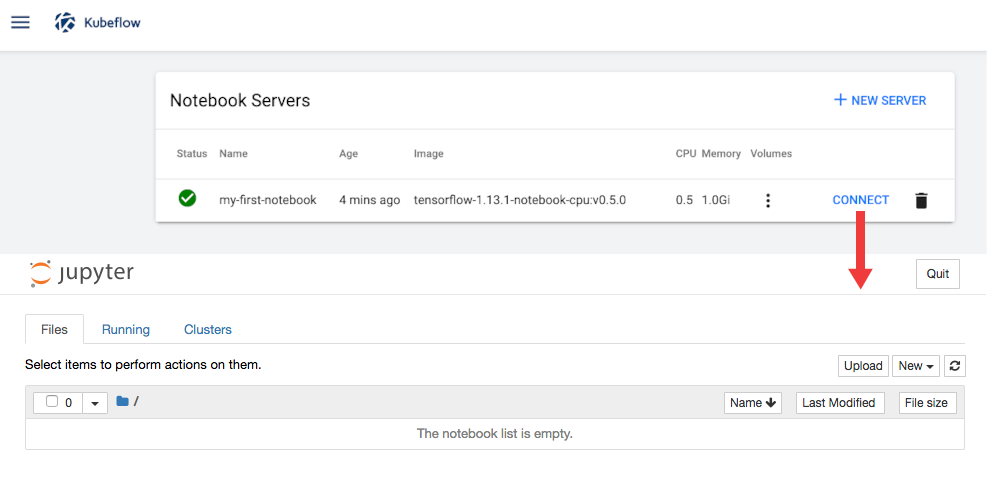
\includegraphics[width=.9\linewidth]{./img/solution1.png}
\end{center}
\subsection*{Solution 2a}
\label{sec:org1e39bb3}
\begin{center}
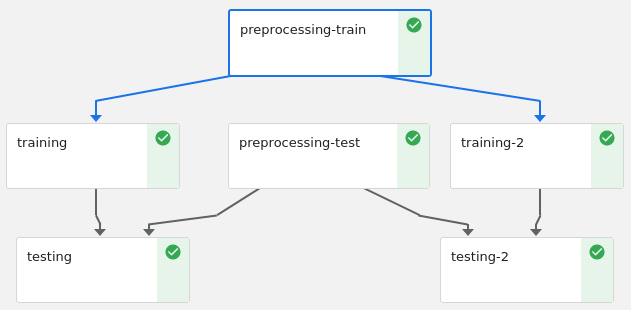
\includegraphics[width=.9\linewidth]{./img/solution2a.png}
\end{center}
\subsection*{Solution 2b}
\label{sec:org8cea593}
\begin{center}
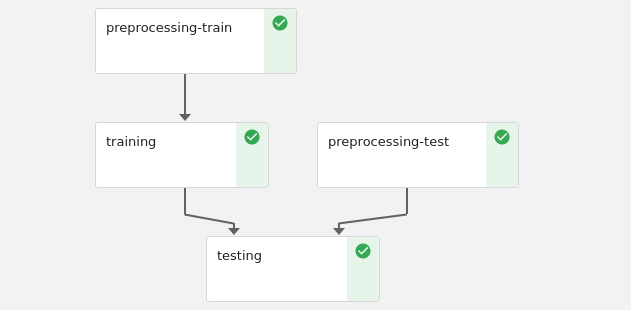
\includegraphics[width=.9\linewidth]{./img/solution2b.png}
\end{center}
\subsection*{Performance}
\label{sec:orga266aaa}
\begin{center}
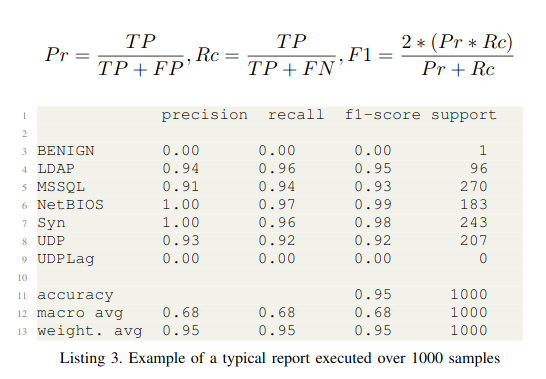
\includegraphics[width=.9\linewidth]{./img/performance.png}
\end{center}
\subsection*{Timing}
\label{sec:org705ee67}
\begin{center}
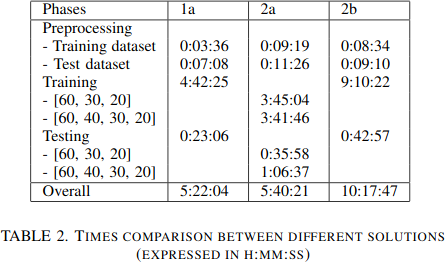
\includegraphics[width=.9\linewidth]{./img/timing.png}
\end{center}
\subsection*{Comments}
\label{sec:org1bc1c0a}
\begin{itemize}
\item Significant reductions in times with concurrency
\item Small overhead on component initialization and management
\item Pipeline implementations are overall slower than the notebook
execution
\begin{description}
\item[{Warning}] Your CPU supports instructions that this TensorFlow
binary was not compiled touse: SSE4.1 SSE4.2
\end{description}
\end{itemize}
\subsection*{Conclusions}
\label{sec:org67e09be}
\begin{description}
\item[{Dataset}] Highly inbalanced
\begin{description}
\item[{TODO}] Deal with the inbalance (e.g. resampling)
\item[{TODO}] Use of raw data
\end{description}
\item[{Kubeflow}] Portability/reusability and concurrency
\begin{description}
\item[{TODO}] TensorFlow with full instruction set support
\item[{TODO}] Increase the level of concurrency
\item[{TODO}] Evaluate Kubeflow Katib for hyperparameter tuning
\end{description}
\end{description}
\end{document}
